\section{Switching to an ARM Controller}
The obvious next evolution step would be to include the BMA Sensor into the analog Version. But since the ATMega328P has a lot of reserved pins there are not enough usable pins to supply the BMA and the 42 LEDs (only one Pin was missing). So there were a few possible solutions
\subsection{AVR Controller in a bigger Package}
Regarding the Software this would be the easiest Varaint to go with.
But there are a few disadvantages of the AVR Controller.
\begin{itemize}
	\item a larger Package requires more PCB Space
	\item it requires 6 Pins for ISP programming
	\item it has a bigger power consumption than modern Controllers
	\item modern Controllers are faster
	\item it is an old Controller ;-)
	\item there is no technical challenge 
\end{itemize}
So this was not the final solution.
\subsection{Atmel SAM}
I started with the Atmel SAM Controller, because I liked the experience with Atmel Controllers so far. For a comparison of Microcontrollers there is a great article from Jay Carlson \url{https://jaycarlson.net/microcontrollers/}. The advantage of the Atmel SAM Controllers are there are a lot of open source Tools which could also be used out of a makefile, so the projectsrtucture is very easy to create. All the Configuration and the Bootupsequence is generated by the Atmel Start utility. \url{https://start.atmel.com/}. The feature i liked the most is the SERCOM Interface.A SERCOM interface could be used for various serial Interfaces (UART, I2C, SPI...), the biggest advantage is that all thepins could be multiplexed with each other.

Therefore i created a Evaluationboard i could start playing around with:
\url{https://github.com/sulkith/devboards/tree/master/ATSAML22G18A_LowPowerArm}

Once the Board arived i encountered the first problem. The files generated by the Atmel Start utility are licensed under the ASF license. And since i'm no lawyer, i couldn't really decide if it is safe to use these files in an open-source project like this one. So i decided to build a wrapper, which would unpack the Package generated by the Atmel Start utility and include the files in my project Structure (\url{https://github.com/sulkith/devboards/blob/master/ATSAML22G18A_LowPowerArm/Software/AtmelStart/AtmelStartIntegrate/importAtzip.sh}). But as soon as you need to change some code in the Startup or in the drivers the whole process is not working anymore.

But since in the early stages one has to change a lot of settings in the configurator and include it back in my code. So the whole Workflow is some kind of clumpsy. And i got a bit sick of changing a Setting and taking one or two minutes to change a single option. So i was looking for a solution where the whole process is smoother.

\subsection{STM32}
So a few colleques suggested to go for a STM32 Controller because the STMCubeIDE is very smooth and all configurations are done inside the IDE.Afterwards the Code is directly generated. A big plus point was that in the copiright notice it is explicitely stated, that you are allowed to redistribute the software if you mention the original source(this is automatically done in the header of every file). So using it for an open source project doesn't seem to be a problem.

\subsubsection{STM32L053R8}
To start with the ecosystem i went for a Nucleo-L053R8 development board with a lowpower Cortex M0+. It took me about half an hour to get the I2C running. So the IDE is great and easy to use. The Controller used on the Board is featuring a on-chip RTC which is also running in all Low-Power modes including Standby mode. So all the Timekeeping wor the wrist watch could be done completely by the chip. There is also a RTC-Clibration feature, which could be used to syncronize the deviation of the Crystal with a high precision frequency source. 
Sadly the STM32L053R8 Controller is not available in a QFN32 Package.

\subsubsection{STM32L432K} 
While searching for a replacement for the STM32L053R8 i came across the STM32L432K Controller, with a Cortex M4 Core, which is also featuring a Shutdown mode with only about 400 nA with the RTC running. So the Watch will consume very low power. A Wakeup is also possible by the Wakeup pin, which could be connected to the BMA Controller to wake up the Controller on wrist tilt or double-tap. There are enough pins for using the Wakeup Pin, SPI, SWD-Debugging and supplying all 42 LED for the analog version.
So from the Hardware point of view everything is fine.

\paragraph{Binary PCB}
Sinc the ST QFN Package looks like a big black box i also placed the BMA456 sensor, which also looks like a black box right next to it for a more PCB like look.
\begin{center}
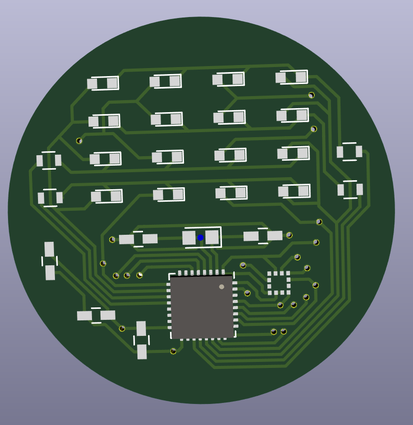
\includegraphics[width=0.45\textwidth]{../Schematics/Schematics_STM/Watch.png}
\end{center}
\paragraph{The Boot Pin}
When the first PCBs arrived it was very easy to get them working, but when the Debugger was not connected sometimes the controller wasn't booting correctly and was displaying strage things on the LED. When connecting to the controller without a reset one could identify the courrent all stack. And the address was in the section of the ST Bootloader. So the obvious suspect was the Boot Pin, the pin was floating in the initial PCB design and this is a bad Idea. In the first Prototype this was fixed by connecting it directly to the neighbouring ground pin. For the next version there will be a resistor pulling it to ground.

Since the Watch was working now it was time to get the crystal calibration working. But since the controller only has a 32 Pin Package the Calibration Pin is not available in the footprint. 

\paragraph{Calibration}
A Workaround for the missing calibration feature was to use the Timer in frequency counter mode with the LSE clock(External Crystal) connected to the Clock pin. So the Input timervalue will be saved on each Signal edge, after two edges the difference could be calculated. For an input Frequency of 1Hz the difference has to be exactly 32768. To increase the accuracy was the presacaler was set to the maximum value of 8. So the value has to be exactly 8*32768. To further increase the accuracy the whole process will be repeated 20 Times and then the average deviation will be calculated. From this deviation the correction value per 1 ppm could be calculated. But after the calibration procedure the Watch was still not very acurate.

\paragraph{Load Capacitance}
While searching for the source of the Clock Deviattion i came across the Application Note 2867
\url{https://www.st.com/resource/en/application_note/cd00221665-oscillator-design-guide-for-stm8af-al-s-stm32-mcus-and-mpus-stmicroelectronics.pdf} Which describes the Design guidelines for oscillators used in combination with STM32 controllers. The crystal used in the Clock is the Abracon ABS05W-32.768 kHz-D. The AN2867 recommends 4pF Load Capacitors for this setup. Till now i used 10pF Capacitors, this could als explain the heavy correction which was needed for the AtMega328P.

So i did a few single measurements to measure the difference of the Changes done. The measurements were done with the same Controller on the same PCB, once with a Battery Supply (2.8V) and once with Power Supply from the Nucleo Board (3,3V), The second change was the Change of the Capacitors from 10pF to 3,9pF (i couldn't get exactly 4pF on the 0603 Package). The Results could be found in the Table below.
\vspace{1cm}

\begin{tabular}{|l|l|l|l|}
\hline
Supply Voltage {[}V{]} & Load Capacitance {[}pF{]} & Frequency {[}Hz{]} & Deviation {[}ppm{]} \\ \hline
2,8   & 10                        & 32549              & -209                \\ \cline{2-4} 
                       & 3,9                       & 32850              & 92                  \\ \hline
3,3   & 10                        & 32548              & -210                \\ \cline{2-4} 
                       & 3,9                       & 32857              & 99                  \\ \hline
\end{tabular}
\vspace{1cm}

So we can conclude that a larger Capacitance slows the oscillator down. The correction needed for the clock was now smaller, but the deviation was still there.

\paragraph{CubeIDE Initialization}
After another few tests i found out there is a relation between Wakeups and the Deviation of the Clock. So the original Proble was every time the Controller is initialized the code generated by the CubeIDE will initialize the whole Clock System. To initialize the driver strength of the LSE Clock the clock has to be stopped, and syncronized again. This Process will delay the RTC Time by about 0,5 seconds.

Therefore i needed to adapt the initialization for the Controller. The function, which was causing the Problems is the \verb!SystemClock_Config()!, if there is a LSE configured it would be initialized. So the obvoius solution would be to disable the LSE. But if the LSE is disabled the RTC would need a Clock, so the RTC was also disabled. The big Problem is if the RTC is disabled in the configuration the HAL Driver would not be included in the project. So i copied the initialization Function from the code generated without the RTC and renamed it to \verb!SystemClock_Config_without_LSE()! in the Project configuration i disabled the function call to the original \verb!SystemClock_Config()! and called the \verb!SystemClock_Config_without_LSE()! in the usermain instead. Also the RTC initialization had to be rewritten to only initialize the RTC if the LSE is not running. For this task the Function \verb!STM32L4_HAL::HAL_driverInit()! was introduced. This Function checks if a RTC clock source is set. The clock source is set in the \verb!RCC_BDCR! register, which resides in the backupdomain of the STM and therefore is not cleared by a reset. So the initialization will be only done once when the Battery is inserted.

\paragraph{Analog PCB}
Since the STM32L432K has more usable pins than the Atmega328P it was also possible to route a PCB with the BMA Sensor and the Analog Watchface.
The space for the Analog Watchface was already very tight without the BMA Sensor. With the Sensor it got extremely tight, so i had to turn the Controller by 45 Degrees. Sadly I was not able to comply with all the Designrules for the BMA Sensor. Now i have a via under the BMA, i think this is very bad for series production, but for me it is working.

\begin{center}
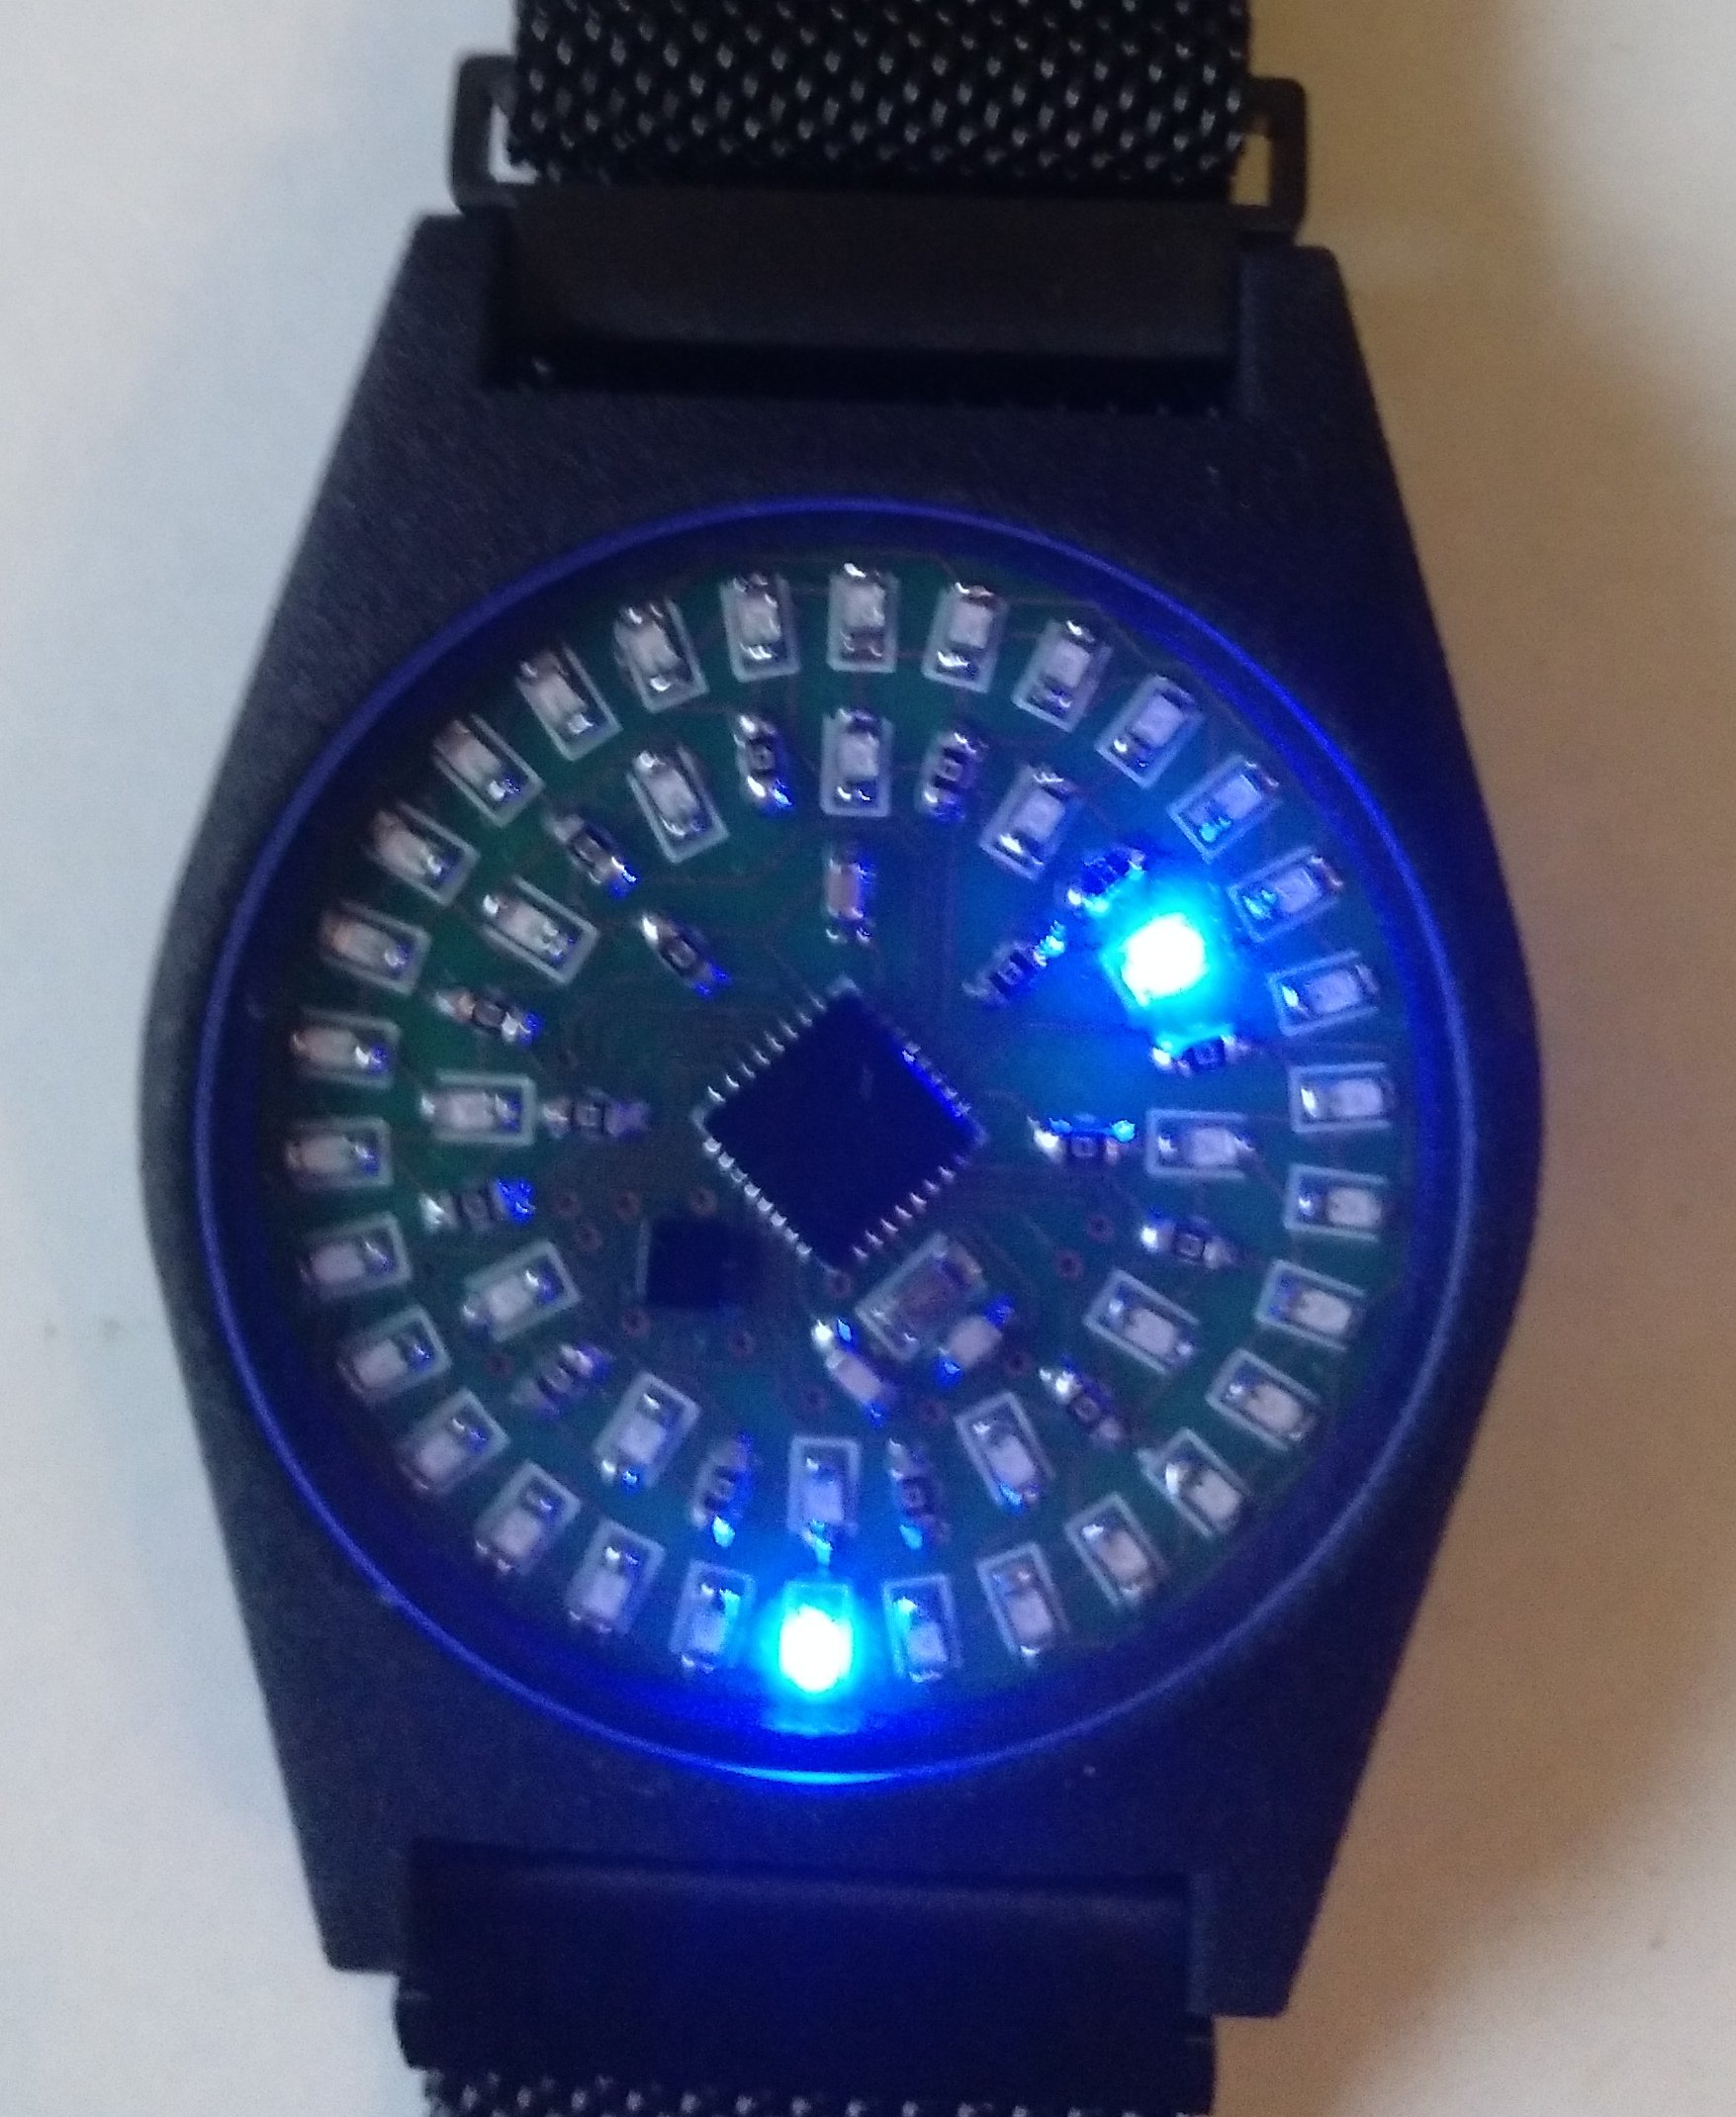
\includegraphics[width=0.45\textwidth]{../Pictures/AnalogSTM.jpg}
\end{center}

\paragraph{Software for the Analog Version}
I wanted to keep the changes on the Software as simple as possible and don't want to maintain two folders with common files between both variants. I created a combined software, which selects the correct \verb!DisplayManager! depending on  the watch variant saved in the flash, right next to the calibration values for the RTC. So i have only one Software, which fits the analog and the binary version of the watch, but i need to specify, via a define in the calibration software, if it is a analog or a binary watch. For further development i also added some defines in the software, which can disable a specific watch variant. This can be used either to save flash memory or to reduce the possible software bugs in the software.
